\documentclass[tikz]{standalone}

\begin{document}
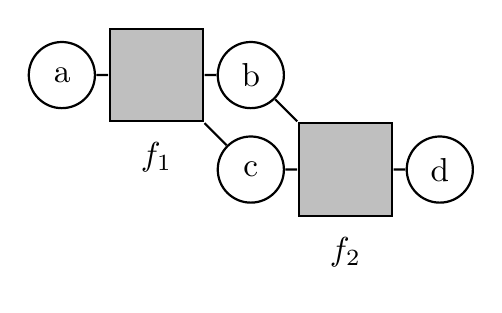
\begin{tikzpicture}[thick, scale=1.2, transform shape]
% define node styles
\tikzstyle{every node}  = [draw, circle, minimum size=7mm]
\tikzstyle{every label} = [draw=none, inner sep=-1pt]
\tikzstyle{factor}      = [draw, rectangle, scale=-1.4, fill=black!25]

% (Aside: Why can we add spaces here, but not above??)
% variable nodes
\foreach \v/\x/\y in {a/1/2, b/3/2, c/3/1, d/5/1}
    \node (\v) at (\x,\y) {\v};

% factor nodes
\foreach \n/\x/\y/\pos in {1/2/2/above, 2/4/1/above}
    \node [factor, label=\pos:$f_\n$] (f\n) at (\x,\y) {};

% edges
\foreach \from/\to in {a/f1, f1/b, b/f2, f1/c, c/f2, f2/d}
    \draw (\from) -- (\to);

\end{tikzpicture}
\end{document}
